\section{Introduction}
One percent of children in the US are born with congenital heart defects [3], which may require surgery to be treated. For doctors to efficiently and effectively plan surgery, it would be useful if a model of the patient's heart can be 3D-printed. Creating a patient-specific heart model requires the 3D MR (or CT) image of the patient to be segmented, which means each voxel (3D pixel) must be labeled with what portion of the heart it belongs to. Traditionally, this means that an expert must manually label each voxel in the image with whether it belongs in the bloodpool, myocardium (muscle), or outside the heart. Currently, patient-specific 3D heart models are underused because it takes around 4-8 hours to manually segment a cardiac MRI image, since each 3D image contains 100-200 slices. Algorithms have been developed to segment the heart in normal adult patients. One of the most popular methods is atlas-based segmentation, which uses a fully segmented heart as a reference and tries to transform the patient's heart to the given reference using image registration. However, atlas-based segmentation methods do not work well on children with congenital heart disease (CHD) due to the irregular location, shapes, and connectivity of the heart substructures, which makes finding the transformation exceedingly difficult. An interactive patch-based method (described in section 2) has been developed to segment images of hearts with CHD, but requires the pre-processing step of finding a bounding box of the heart in the scan.

This paper proposes a method to localize, or find the bounding box of, the heart in 3D images of patients with CHD. Localizing the heart for patients with CHD as opposed to healthy hearts is an additional challenge, because hearts with CHD may have incomplete or missing structures, or structures located in different areas compared to healthy hearts. Therefore, many traditional methods for localizing these images do not work well. The method proposed in this paper attempts to address these challenges.

The method proposed in this paper localizes the heart in patients with congenital heart disease, using random forests. We applied this method on a dataset of 10 patients, by training on 9 and testing on the remaining patient. The percentage error (explained in Section 5.2) was less than 10\% for each patient, and the average percentage error was 4.8\%. These low percentages prove that our method has promise, and may be extended to localize substructures of the heart in the future.

\section{Related Work}
One method for segmentation of the heart in children with CHD is an interactive algorithm based on partial manual segmentation [1]. The user is directed to manually label 10-15 slices uniformly distributed throughout the 3D volume, out of the 100-200 in the image. The algorithm then automatically segments each remaining target slice using its closest reference slices. To segment a patch, which is a rectangle of pixels, the algorithm finds the $k$ most similar patches in the set of reference regions, where ``similarity" depends on patch intensities, gradients, and physical positions. Then each pixel of the target slice is labeled according to a majority vote. This algorithm greatly reduces the amount of time needed to segment a heart to less than 1 hour of manual labelling and 1 hour of algorithm runtime. However, since the algorithm still requires user interaction, it is not fully automatic.

Regression forests, a supervised machine learning technique, have also been shown to do well in the detection and localization of organs. In particular, regression forests have been used to learn the non-linear mapping from voxels directly to organ position and size [2]. The regression forest groups voxels with similar features or similar field of views together, and learns an estimate of the bounding boxes of each organ using the training data. Intuitively, each voxel contributes varying degrees of confidence to the estimates of the location and size of every organ. When applied on real datasets, the forest learns to recognize key indicators (such tips of the ribs or vertebrae) and those pixels provide high confidence estimates of where certain organs are located. Compared to other localization methods such as the Elastix and Simplex methods as well as atlas methods, the regression forest method was superior in accuracy [2]. This paper applies the regression forest methods developed in [2] to children with CHD.

\section{Regression Random Forests}
This paper develops a method to localize the heart in 3D MRI scans of patients with CHD, based on regression random forests. A random forest is a supervised machine learning model that consists of many decision trees. A decision tree is a flow-chart like structure in which each node is a Boolean function on the data's features. The input to a decision tree is a data point and its features, or characteristics, and the output of a decision tree is a label. For example, Figure 1 depicts a decision tree that takes in an image as input and predicts whether it was taken indoors or outdoors. For each data point that passes through the decision tree, as it arrives at each node, the node makes a decision for whether the data point goes to its left child or right child, based on the data point's features. At each leaf node, the data point is classified with a label, which can be binary or multi-class classification. In the case of Figure 1, the label is either ``outdoors" or ``indoors".

\begin{figure}
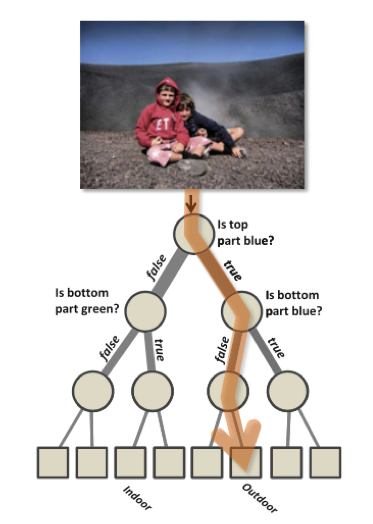
\includegraphics[scale=0.5]{decisiontree.png}
\caption{Diagram of a decision tree for determining whether an image is taken outdoors [2]}
\end{figure}

Our method uses regression forests, which contain regression trees instead of decision trees. Regression trees are the same as decision trees except that each leaf node contains a regression model instead of a classification model. A regression model outputs a number of vector of numbers, instead of a discrete label. Therefore each leaf node would predict a regression value instead of a classification label. The method in this paper uses regression trees instead of decision trees because we want to predict the location of a bounding box, which is modeled as a continuous variable rather than a discrete one.

\begin{figure*}
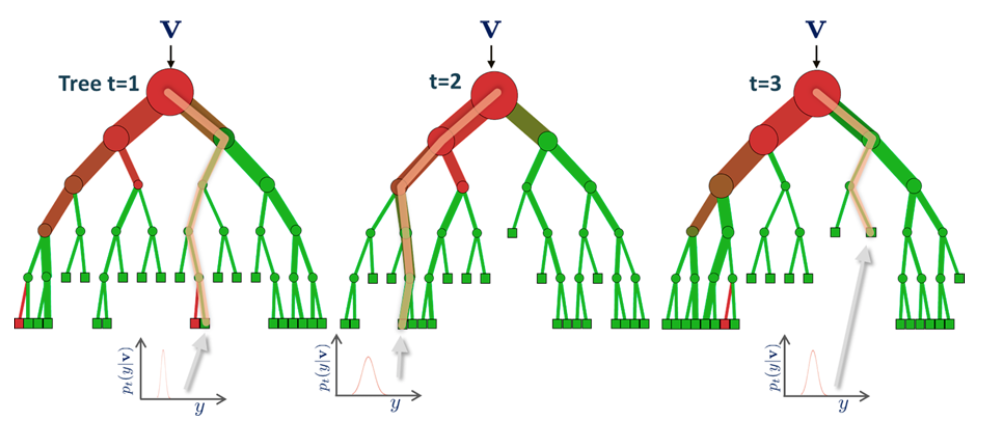
\includegraphics[scale=0.45]{regressionforest.png}
\caption{Diagram of a regression forest consisting of 3 trees and a depth of 5 [2]}
\end{figure*}

\begin{figure*}
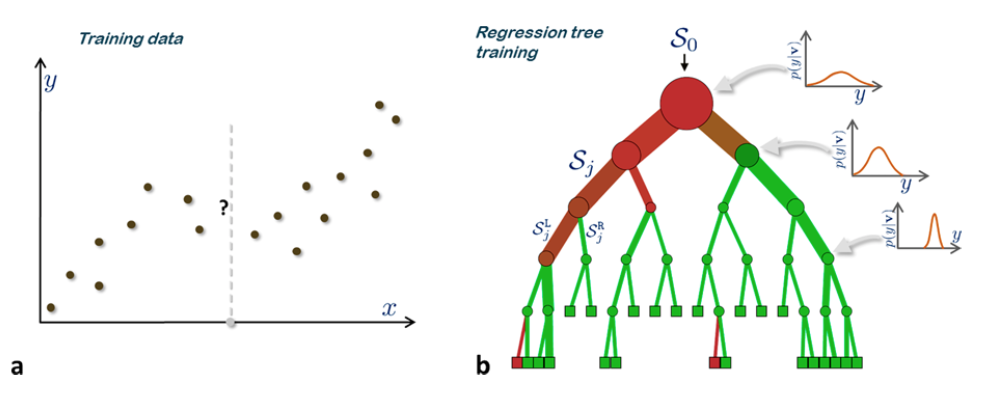
\includegraphics[scale=0.45]{regressiontraining.png}
\caption{Training a regression tree: a) depicts a potential split function, where $x$ and $y$ are features of the training data, and b) depicts the regression tree with Gaussian models fitted at each node [2]}
\end{figure*}

A regression forest is produced by aggregating many regression trees. Figure 2 shows a regression forest consisting of 3 trees. For each tree, a data point can be seen passing through the tree's branches and down to the leaf node, where it is put into a regression model. In the case of this paper, the regression model at the leaf nodes is a Gaussian distribution.
  
A regression forest can be trained by individually training its regression trees. The training of each tree contains some degree of randomness, which significantly reduces training time but leads to a sub-optimally trained tree. Forests containing many such trees recover accuracy and can be trained in parallel.

Training a tree involves determining features to split at each node, and training a regression model at each leaf. Regression trees are trained by minimizing some loss function at each node. We maximize information gain as the method for choosing each split node's split function, because it will choose the function that will best separate the dataset. Information gain is expressed in terms of entropy, which can be thought as a measure of randomness in the dataset. Maximizing information gain is equivalent to minimizing the randomness in the two datasets produced by the split function. Intuitively, this results in greedily training the tree such that each time the tree branches, we get clusters of data points that have similar features and will therefore produce similar output values. The split function at each node is chosen using the following equation:

\begin{equation}
  \theta^* = \text{argmin}_{\theta}(H(S) - \frac{|S^L|}{|S|} H(S^L) - \frac{|S^R|}{|S|} H(S^R))
\end{equation}
where $S$ is the training data that has reached that node, $\theta$ denotes the parameters of the function being considered at the split node, $\theta^*$ is the optimal parameter, $S^L$ is the subset that will go to the left node, and $S^R$ is the subset that will go to the right node, and $H(S)$ is the entropy of a dataset $S$ fitted with a multivariate Gaussian model, given below:

\begin{equation}
  H(S) = \frac{1}{2} n \log(2\pi e  |\Sigma|)
\end{equation}

where $\Sigma$ is the covariance matrix of a Gaussian model that is fitted to the dataset at the node.

To train a regression tree, we greedily choose the split functions at each node. At each node, $K$ features are randomly selected, and the feature that maximizes the information gain given above is chosen as the split function for that node. We only consider $K$ features at a time because it is too computationally intensive to consider all the possible features for the split function. Figure 3 depicts how a selected feature divides the training set. Training a tree terminates either when the maximum tree depth has been reached, or when the information gain is less than some threshold value. After each regression tree is trained, the set of these trees becomes the regression forest. The introduction of randomness in feature selection is meant to prevent overfitting: each tree is a weak learner, but the aggregation of many randomly trained weak learners should be a strong learner. Training many weak learners in parallel is also computationally much faster than training one strong learner such as a deep regression tree.

Three hyper-parameters determine the structure of the regression forest: $T$ is the number of trees, $D$ is the maximum tree depth, and $K$ is the number of features being considered at each node.

Once a regression forest is trained, it can make predictions on new data points by running the data point through each of the regression trees until it reaches a leaf node, and predicts the output value using the regression model at that leaf node. Finally, we combine the outputs of each regression tree, which is typically an average over all the trees, to produce the output of the regression forest.

\section{Method}
\subsection{Regression Forests for Localization of the Heart}
We trained a regression forest to predict the location of the bounding box of the heart given an MRI scan of a patient with congenital heart disease. Instead of running each entire image through the tree, we run features for each voxel through the tree, and each of those will define a distribution of where the bounding box is according to that voxel. Our method for calculating features for each voxel is described in Section 4.2. We then aggregate the distributions from each voxel to get a final distribution for where the bounding box should be.

A bounding box is given by a 6-dimensional vector: $(x_1, x_2, y_1, y_2, z_1, z_2)$. Here, $x_1$ and $x_2$ denote the $x$-values of the two faces of the bounding box that are perpendicular to the $x$-axis, where $x_1$ is the smaller of the two values, and $y_1, y_2, z_1, z_2$ are similarly defined for the other axes. Figure 4 shows the ground truth bounding box of a patient's heart as viewed from three different axes.

\begin{figure*}
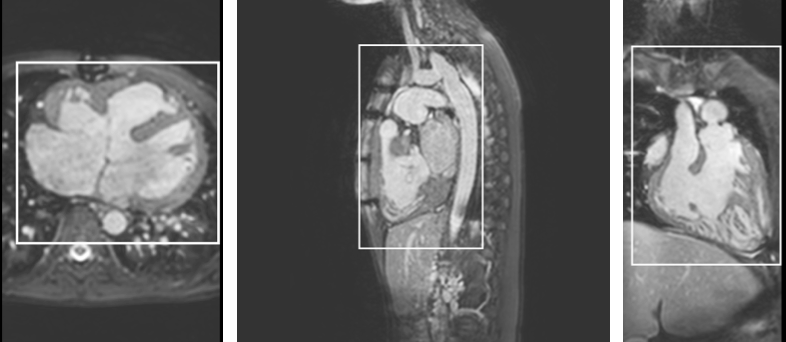
\includegraphics[scale=1.0]{boundingboxes.png}
\caption{Ground truth bounding box of patient 0, as viewed from three different axes}
\end{figure*}

For each voxel location $\mathbf{p}=(p_x, p_y, p_z)$ that we run through the regression forest, we calculate its offset from the bounding box $\mathbf{b}$:
\begin{equation}
  d(\mathbf{p}, \mathbf{b}) = (x_1, x_2, y_1, y_2, z_1, z_2) - (p_x, p_x, p_y, p_y, p_z).
\end{equation}
The Gaussian model fitted at each node is then a 6D Gaussian, representing the voxel's predicted offset from the bounding box. Each of the leaf nodes therefore has a distribution of the voxel's offset from the bounding box, not the bounding box locations themselves. We use relative offsets because the absolute positions of structures within the heart will be different for different scans. Recording relative offsets also captures the relationships between the locations of important image characteristics and the bounding box of the heart.

At testing time, to produce predictions for the bounding box of a heart given a new 3D image, we take each voxel in the image and run it through the regression forest. For each voxel, we determine the predicted offset from the bounding box according to that voxel by combining the Gaussian distributions resulting from each tree in the forest. Then, we add back the voxel's location to get the distribution of the predicted absolute location of the bounding box. Finally, we average the distributions from each voxel to form the final predicted distribution of the absolute bounding box of the heart.

\subsection{Feature Selection}
As mentioned previously, at each split node, $K$ features are chosen randomly for consideration as the split feature. Each feature is calculated as the mean intensity of voxels in a rectangular box, that is located at some offset to the voxel. Figure 5 is a visualization of such a feature. Each feature is governed by the following parameters: $a$ is the offset to the center of the box, which is a 3D vector, and $b$ is the size of the box, which is also a 3D vector. Each dimension of the box must be odd, to ensure that the center of the box is on a lattice point. A feature is calculated with the following equation:

\begin{figure}
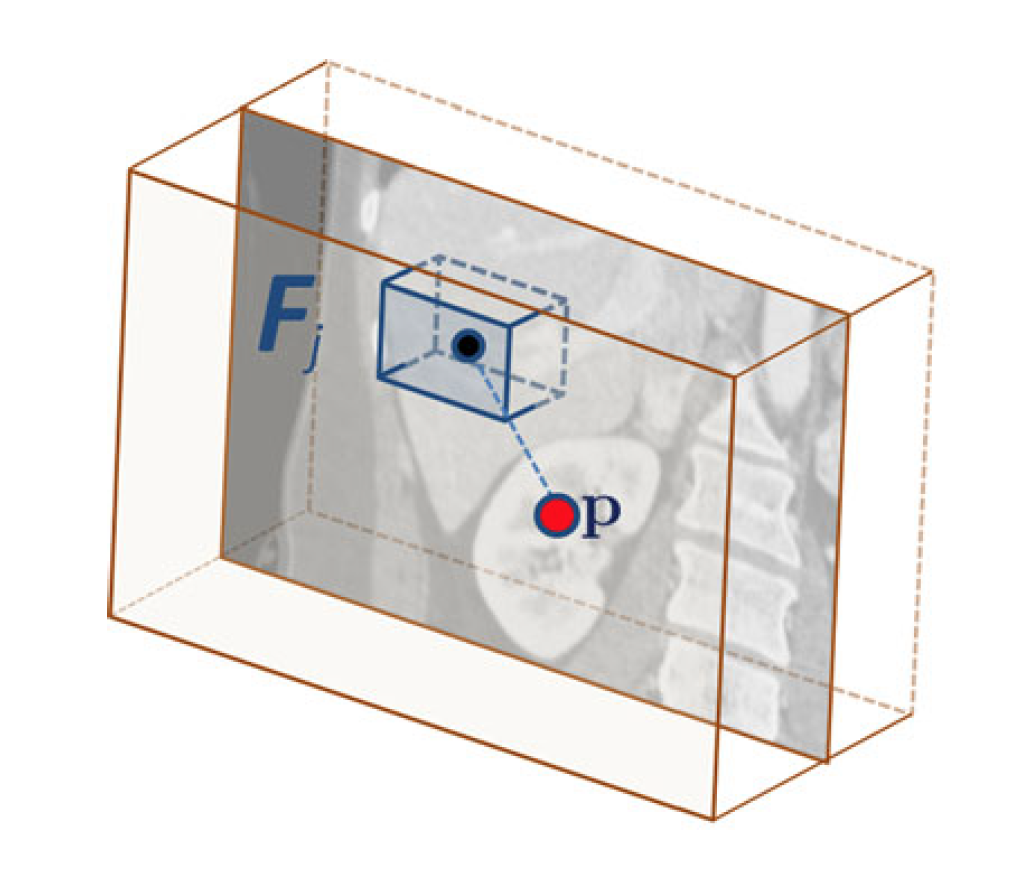
\includegraphics[scale=0.4]{feature.png}
\caption{A randomly selected feature, which is the average intensity over a box of voxels located some offset away from $p$ [2]}
\end{figure}

\begin{equation}
  F_{a, b} = \frac{1}{|B_{a,b}|} \sum_{v \in B_{a, b}} J(v)
\end{equation}
where $B$ is the set of voxels that lie in the box that is described by an offset of $a$ and a box size of $b$, and $J(v)$ describes the intensity at the voxel $v$. These features are selected because the presence of certain features in the image, such as bright or dark spots, can hint at where the heart is. Therefore, having an especially high or low mean intensity of voxels at a specific offset can contribute a good prediction as to where the heart may be.

To generate a random feature, we sample $a$ and $b$ from uniform distributions. Each element of $a$ is sampled from a uniform distribution from 0 to a fixed fraction of the size of the image in that dimension. Each element of $b$ is sampled from a uniform distribution of 1 to $2k+1$ for some $k$. Currently the parameters are set at $\frac{1}{6}$ of the image size for $a$, and $k = 5$ for $b$. 

\section{Results}
\subsection{Dataset}
The dataset consists of 3D cardiovascular MRI scans of 10 different patients, which have a variety of congenital heart defects. Manual segmentation was performed on each of the 10 scans, taking around 8 hours each. Image dimension varied across patients, but was 340 x 340 x 140 on average, after resampling the voxel size to 1 x 1 x 1 mm. To evaluate the performance of the proposed method, the regression forest was trained on 9 patients and tested on the remaining patient. 

\subsection{Localization Error}
To produce a prediction of the bounding box, we use maximum-likelihood estimation: each element in the bounding box vector is produced by sampling the distribution and finding the value with the maximum probability. We calculate two types of errors: the first is the voxel error, which is the L1 norm of the error between the true bounding box and the calculated most likely bounding box. The second is the percentage error, which is the L1 norm of the same error with each element in the vector expressed as a percentage of the image size in that dimension. This allows us to compare the results on test images of all sizes.

For each patient in the dataset, we trained the regression forest using images from the other nine patients, applied the forest on the remaining patient, and calculated the voxel error and the percentage error. Since there is randomness in the training process, the results are averaged over three runs of the algorithm.

\begin{equation}
  E_{\text{voxel}} = \frac{1}{6} \sum_{i=1} ^ {6} |b_i - B_i|
\end{equation}
\begin{equation}
  E_{\text{percent}} = \frac{1}{6} \sum_{i=1} ^ {6} \frac{|b_i - B_i|}{S_{i}}
\end{equation}
where $B$ is the true bounding box, $b$ is the predicted bounding box, and $S_i = (s_1, s_1, s_2, s_2, s_3, s_3)$ where $s_i$ is the size of the image in dimension $i$.
\begin{figure*}
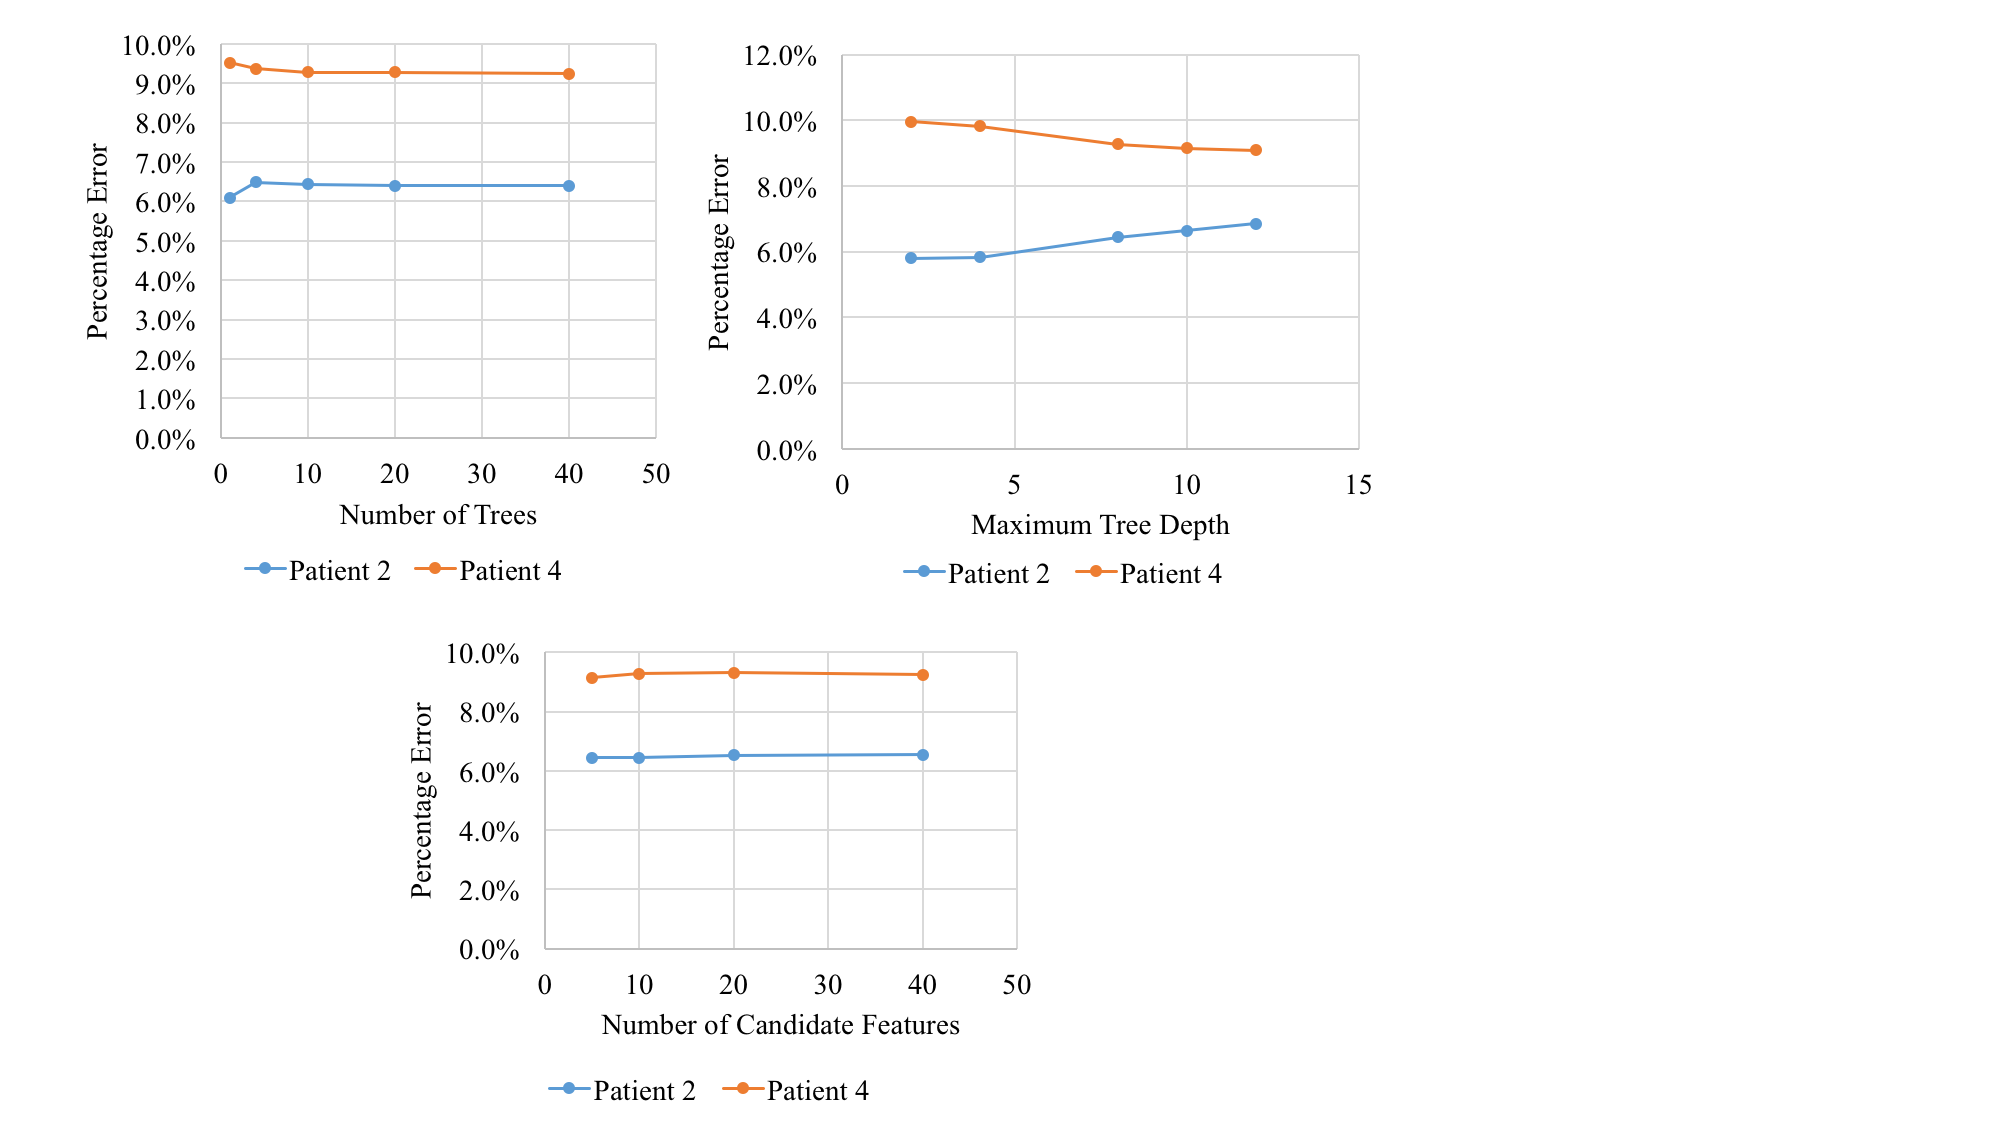
\includegraphics[scale=0.7]{parameters.png}
\caption{Percentage error when performing leave-one-out cross validation on patients 2 and 4, varied over number of trees (top left), maximum tree depth (top right), and number of candidate features (bottom)}
\end{figure*}

\begin{table}
  \caption{Localization errors of ten patients, trained using a regression forest with parameters $T$ = 10, $D$ = 8, and $K$ = 10}
  \label{tab:err}
  \begin{tabular}{p{2cm}p{2cm}p{2cm}}
    \toprule
    Patient Number & Voxel Error (voxels) & Percentage Error (\%) \\
    \midrule
    0 & 6.8 & 2.3\\
    1 & 7.8 & 3.4\\
    2 & 17.4 & 6.4\\
    3 & 31.8 & 8.4\\
    4 & 17.2 & 9.3\\
    5 & 11.7 & 5.7\\
    6 & 9.8 & 3.4\\
    7 & 4.1 & 1.2\\
    8 & 6.6 & 3.4\\
    9 & 11.7 & 4.8\\
    \bottomrule
  \end{tabular}
\end{table}

The results, as shown in Table 1, are obtained by using a regression forest with 10 trees, a maximum tree depth of 8, and 10 randomly selected features at every split node. To speed up training time, the image was sampled at a rate of one voxel for every 9x9x9 cube, which is not expected to impact results significantly because neighboring voxels are highly correlated. As shown in Table 1, the percentage errors are small, with all of them less than 10\%. The average percentage error over all the patients was 4.8\%. Patients 3 and 4 had relatively worse percentage errors, which is what we expect because both patients have severe defects and their images are low resolution, making it harder to predict a bounding box.

\subsection{Parameter Sensitivity}
To investigate the effect of varying the regression forest parameters, we varied three different parameters and observed the percentage error while testing on patients 2 and 4, and training on the remaining 9 images. The three different parameters are number of trees ($T$), maximum tree depth ($D$), and number of features considered at each split node ($K$). We mainly focused on testing with patient 2 and 4, because the heart of patient 2 has relatively normal anatomy while patient 4's scan is low resolution and has severe defects.

\subsubsection{Number of Trees} We varied $T$ while keeping $D=8$ and $K=10$. As shown in the top left graph in Figure 6, the number of trees does not seem to affect percentage error for either patient. This is somewhat unexpected because larger ensembles usually increase accuracy compared to very small ensembles.

\subsubsection{Maximum Tree Depth} We varied $D$ while keeping $T=10$ and $K=10$. As shown in the top right graph in Figure 6, the maximum tree depth seems to affect percentage error slightly for both patients. For patient 2, increasing tree depth resulted in a higher percentage error, while for patient 4 increasing tree depth resulted in a lower percentage error. This is somewhat unexpected because increasing tree depth should usually decrease percentage error, and not have opposite effects in different patients. However, this can be explained because a shallower tree will do well in a normal case and badly in an abnormal case, whereas a deeper tree tries to account for anomalies and therefore will do better in abnormal cases. Patient 2 is a more normal case while patient 4 has severe defects, which supports the above reasoning.

\subsubsection{Number of Features Considered at Each Split Node} We varied $K$ while keeping $T=10$ and $D=8$. As shown in the bottom graph in Figure 6, the number of candidate features at each split node does not seem to affect percentage error for either patient. This is somewhat unexpected because having too little candidate features should increase the error of a trained tree, and having too many candidate features will contribute to overfitting and increase the error of a trained tree. However, we may not be exploring near the optimal value of the parameter which may explain the lack of a trendline. 

\subsection{Discussion}
Our results while varying parameters are somewhat inconclusive because we expected the parameters to affect the results more than we found. This may be because we only ran 2-3 trials per patient for each parameter setting. We also may be exploring a suboptimal region of the parameter space, and in the future we should investigate a wider range of parameters.

\section{Conclusion and Future Work}
We have demonstrated that regression forests can locate bounding boxes of the heart to a reasonable degree of error (less than 10\%), for patients with CHD. The error rate depends slightly on the parameters of the regression forest, especially maximum tree depth. We have demonstrated the feasibility of the algorithm through testing and training on a dataset of 10 patients.

A logical next step would be to extend the algorithm to identify bounding boxes of substructures of the heart, which would be a good pre-processing step to segmenting a 3D image of the heart. Another improvement would be to parallelize the code, exploiting the parallel nature of random forests to speed up the algorithm and allow for the forest to have more trees or increase depth. These extensions would further benefit the process of creating a 3D-printed heart model.

\section{Bibliography}
[1] D. Pace, A. Dalca, T. Geva, A. Powell, M. Moghari, P. Golland, Interactive Whole-Heart Segmentation in Congenital Heart Disease

[2] A. Criminisi, J. Shotton (eds.), Decision Forests for Computer Vision and Medical Image Analysis, Advances in Computer Vision and Pattern Recognition

[3] ``Congenital Heart Defects (CHDs)." Centers for Disease Control and Prevention. Centers for Disease Control and Prevention, 01 Aug. 2016. Web. 14 May 2017.

